% XeLaTeX can use any Mac OS X font. See the setromanfont command below.
% Input to XeLaTeX is full Unicode, so Unicode characters can be typed directly into the source.

% The next lines tell TeXShop to typeset with xelatex, and to open and save the source with Unicode encoding.

%!TEX TS-program = xelatex
%!TEX encoding = UTF-8 Unicode

\documentclass[11pt]{article}
\usepackage{geometry}                % See geometry.pdf to learn the layout options. There are lots.
\geometry{margin=1.7cm,top=1.0cm,bottom=2.0cm}
\geometry{letterpaper}                   % ... or a4paper or a5paper or ... 
%\geometry{landscape}                % Activate for for rotated page geometry
\usepackage[parfill]{parskip}    % Activate to begin paragraphs with an empty line rather than an indent
\usepackage{graphicx}
\usepackage{amssymb}

\usepackage[compact]{titlesec}
\titlespacing{\section}{0pt}{2ex}{1ex}
\titlespacing{\subsection}{0pt}{1ex}{0ex}
\titlespacing{\subsubsection}{0pt}{0.5ex}{0ex}

% use case command
\usepackage{booktabs}

\newcommand\addrow[2]{#1 &#2\\ }

\newcommand\addheading[2]{#1 &#2\\ \hline}
\newcommand\tabularhead{\begin{tabular}{lp{0.8\linewidth}}
\hline
}

\newcommand\addmulrow[2]{\begin{minipage}[t][][t]{2.5cm}#1\end{minipage}% 
   &\begin{minipage}[t][][t]{0.8\linewidth}
    \begin{enumerate} #2   \end{enumerate}
    \end{minipage}\\ }

\newenvironment{usecase}{\tabularhead}
{\hline\end{tabular}}

% Will Robertson's fontspec.sty can be used to simplify font choices.
% To experiment, open /Applications/Font Book to examine the fonts provided on Mac OS X,
% and change "Hoefler Text" to any of these choices.

\usepackage{fontspec,xltxtra,xunicode}
\defaultfontfeatures{Mapping=tex-text}
\setromanfont[Mapping=tex-text]{Hoefler Text}
\setsansfont[Scale=MatchLowercase,Mapping=tex-text]{Gill Sans}
\setmonofont[Scale=MatchLowercase]{Andale Mono}

\title{Final Project Specification: Miller's Hollow Online}
\author{Team \textbf{Miller's Hollow}
\\Yiyun Yao(yiyuny) \& Jin Wang(jinw2) \& Shangjie Chen(shangjic)}
\date{}                                           % Activate to display a given date or no date

\begin{document}
\maketitle

\section{Functionality}
\subsection{Not in a Game}
\subsubsection{Authentication}
\begin{enumerate}
\item
Login: Registered Users may login to the website by correct username and password, and get authenticated and authorized
\item
Register: Unregistered Users may register to the website by providing username, password and email
\item
Activate Account: Registered User may activate the account by click the activation link in the email automatically sent when successfully registered
\item
Logout: Authenticated User may logout the website
\item
Change Password: Authenticated User may change the password by correct current password
\item
Reset Password: User who forget their password may reset the password by providing the email correspond to the account
\item
Reset Password Confirm: User may set their new password by click the link in the email automatically sent when password is successfully reset
\end{enumerate}

\subsubsection{Profiling \& Setting}
The main function is like the Figure \ref{fig:func-settings}.

\begin{enumerate}
\item
Editing User Information: Authenticated User may change the first name, last name and email
\item
Upload avatar: Authenticated User may upload a picture to change the avatar
\item
Set preference game: Authenticated User may set the preference game in the settings to skip the game choose phase in build game and matching game
\item
Set waiting time: Authenticated User may set the waiting time in the settings to change the default waiting time before every speech starts
\item
Set Music, Display and Log settings: Authenticated User may set the music volume, display settings(turn on/off camera of other user in case the network is not good enought) and log verbosity in the settings
\end{enumerate}

\subsubsection{Game Mode}
The main function is like the Figure \ref{fig:func-index}.

\begin{enumerate}
\item
Matching Game: Authenticated User may start a matching game where different unrelated players attend
\item
Build Room Game: Authenticated User may build a room game where friends are invited to play game together; in the mean time, a share token is generated for other users to join
\item
Join Room Game: Authenticated User may join a room game by a share token
\end{enumerate}

\begin{figure}
\centering
\begin{minipage}{.5\linewidth}
\centering
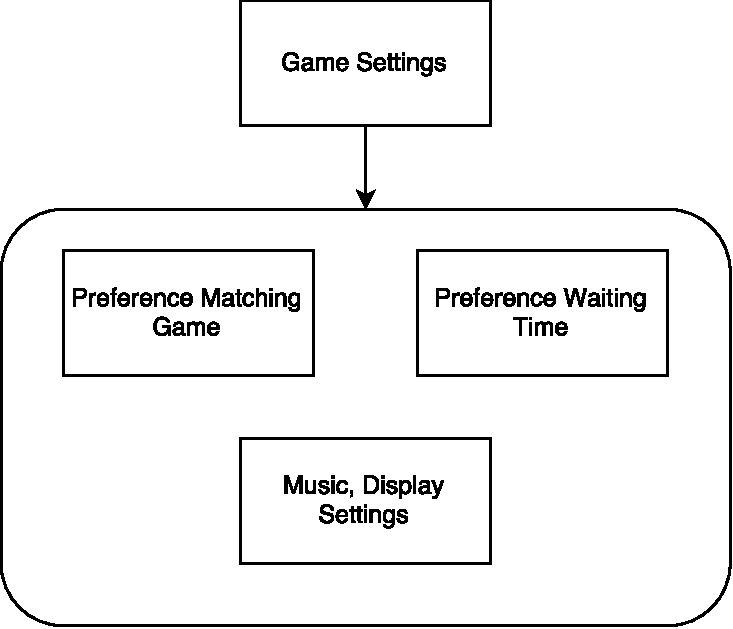
\includegraphics[width=.9\linewidth]{func-settings.pdf}
\caption{Functionality: Profiling \& Setting}
\label{fig:func-settings}
\end{minipage}%
\begin{minipage}{.5\linewidth}
\centering
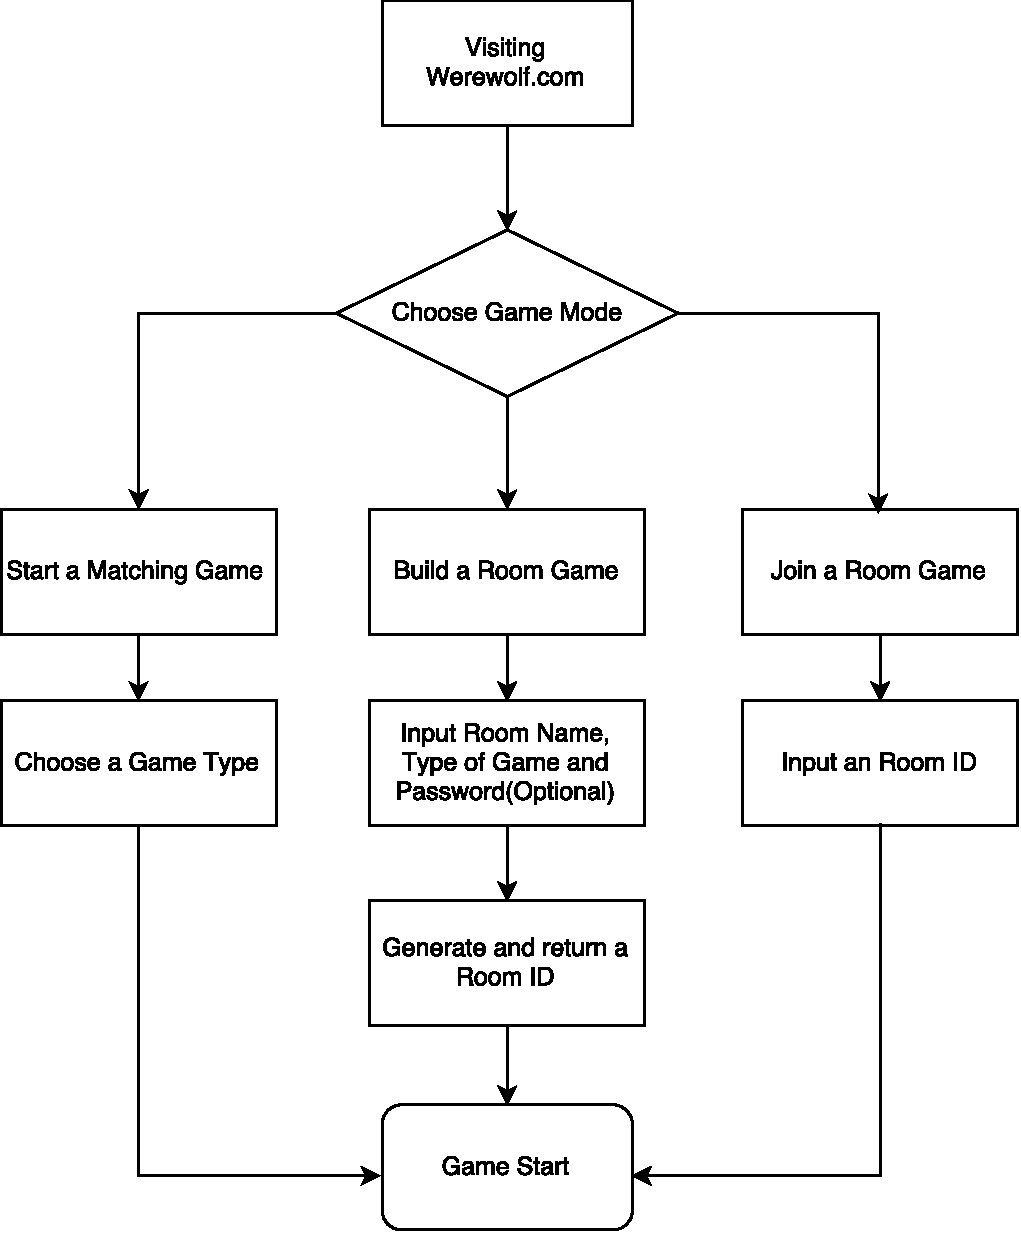
\includegraphics[width=.9\linewidth]{func-index.pdf}
\caption{Functionality: Game Mode}
\label{fig:func-index}
\end{minipage}
\end{figure}

\subsubsection{Room Member}
The main function is like the Figure \ref{fig:func-inroom}.

When Authenticated User join a Room Game, he/she automatically becomes a Room Member
\begin{enumerate}
\item
Change to empty seat: Room Member may change the seat to a new one if it is empty
\item
Leave the room: Room Member may leave the room by clicking the Leave Button
\item
Chat: Room Member may chat in the room and the message can be seen by all the Room Members
\item
Get ready: Room Member may get ready by clicking the Ready Button(when all the Room Member is ready, the Room Owner can Start the game)
\item
Cancel ready: Room Member who is ready may cancel it by clicking the Cancel Button
\end{enumerate}

\subsubsection{Room Owner}
The main function is like the Figure \ref{fig:func-inroom}.

Room Owner have the functionality of Room Member from 1 to 3. A Room Member can be selected as a Room Owner by the previous Room Owner. The original one is the user who build the room. A Room Game can only have one Room Owner. Room Owner has the extra functionalities as follow.
\begin{enumerate}
\item
Set a Room Member as Room Owner: Room Owner may choose another user as the new Room Owner
\item
Kickout Room Member: Room Owner may kickout Room member
\item
Start Game: Room Owner may start the Room Game by clicking Start Button when all the Room Member is ready
\end{enumerate}

\subsubsection{Achievements \& Tasks}
The main function is like the Figure \ref{fig:func-tasks}.

\begin{enumerate}
\item
Tasks: Authenticated User may receive one task a day automatically in the Achievements \& Tasks Board, and get awards by completing it. One user can hold three tasks at max
\item
Exchange task: Authenticated User may exchange a task one day, the new one will be different from the old one
\item
Winning Rate: Authenticated User may check the winning rate in the Achievements \& Tasks Board
\item
Time Played: Authenticated User may check the time played in the Achievements \& Tasks Board
\item
Level: Authenticated User may check the level in the Achievements \& Tasks Board, which is mainly based on the winning rate and time played. The level is the main dependency of Matching Game
\end{enumerate}

\begin{figure}
\centering
\begin{minipage}{.6\linewidth}
\centering
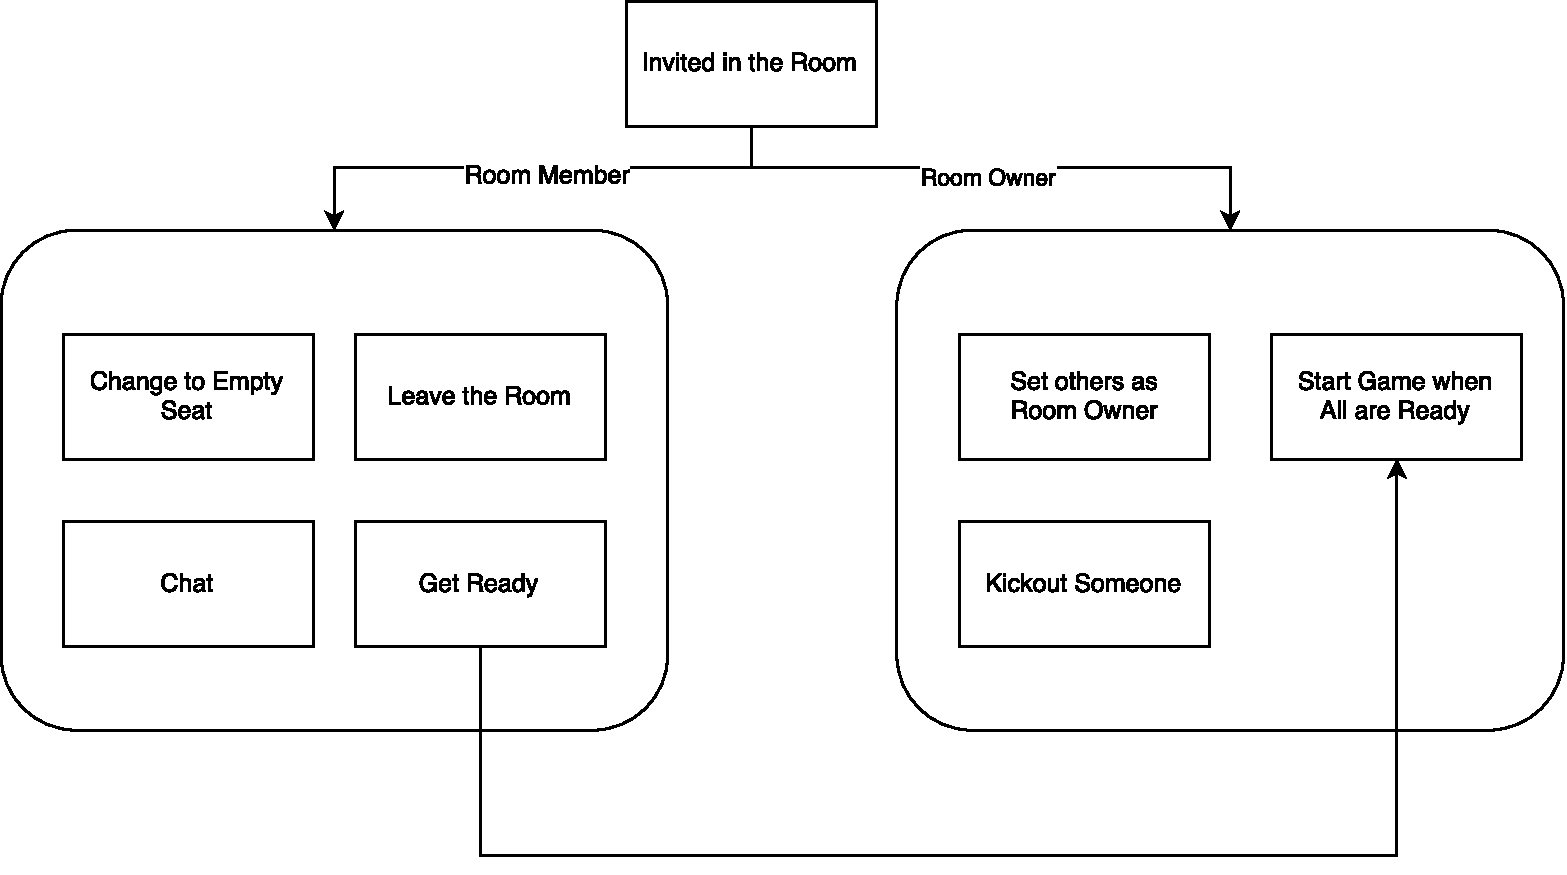
\includegraphics[width=.9\linewidth]{func-inroom.pdf}
\caption{Functionality: Room Member \& Room Owner}
\label{fig:func-inroom}
\end{minipage}%
\begin{minipage}{.4\linewidth}
\centering
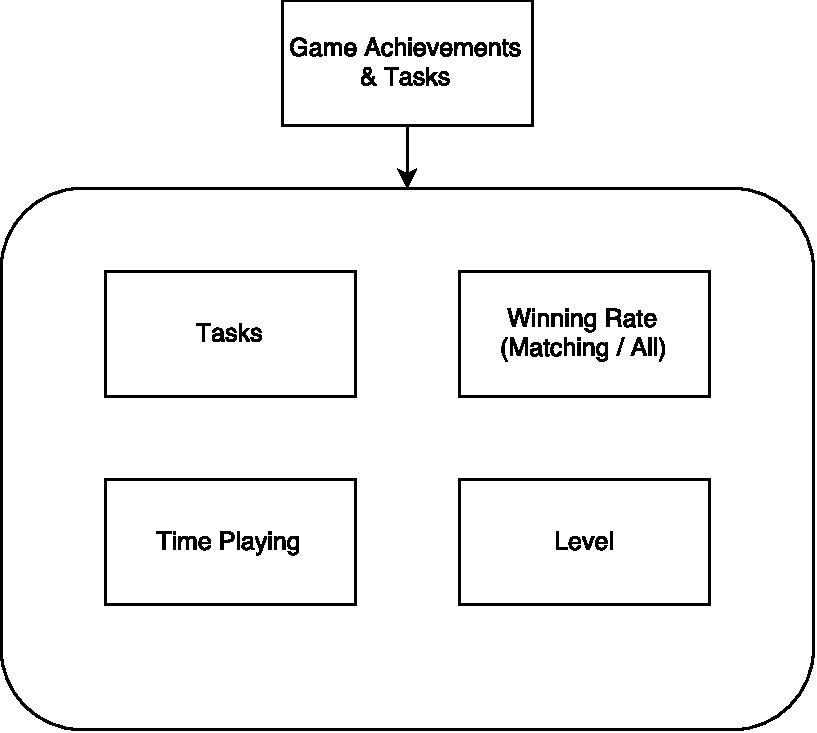
\includegraphics[width=.9\linewidth]{func-tasks.pdf}
\caption{Functionality: Achievements \& Tasks}
\label{fig:func-tasks}
\end{minipage}
\end{figure}

\subsection{In a Game}
When a Game starts, a Room Member automatically becomes a Player
\subsubsection{Get Identity Card}
Before the actual game starts, player can get a identity card which indicates different ability and winning condition in this game. All the identity is shown as follow.

\begin{enumerate}
\item
Villager
\item
Werewolf
\item
Seer
\item
Witch
\item
Hunter
\item
Idiot
\end{enumerate}

\subsubsection{Day Phase}
The main flow chart is like the Figure \ref{fig:func-dayphase}.

\begin{enumerate}
\item
Vote: Player may vote for sheriff or exiling a player by dragging the Hand Button in the menu to the player

\item
Speech: Player may give a speech in his turn. The time of the speech is 1 minute, and player can always end speech in advance

\item
Campaign: In the first morning, player may run for the sheriff by clicking the Hat Button in the menu. The player who doesn't do that, may vote for them. (Sheriff's vote count for 2 instead of 1. If the Sheriff dies, he may decide who will be the next Sheriff)

\item
Perform skill: Player who has a special skill may choose to perform the skill in the appropriate occasion

\begin{enumerate}
\item
Shoot to Kill: Hunter can shoot another player when dying by dragging the Gun Button in the menu to the player
\item
I am Idiot!: Idiot can survive when being exiled automatically
\item
Boom: Werewolf can explode in any stage of the game by clicking the Boom Button in the menu to interrupt the game. In that case, no more user can give a speech and the game comes directly into night phase
\end{enumerate}

\end{enumerate}

\begin{figure}
\centering
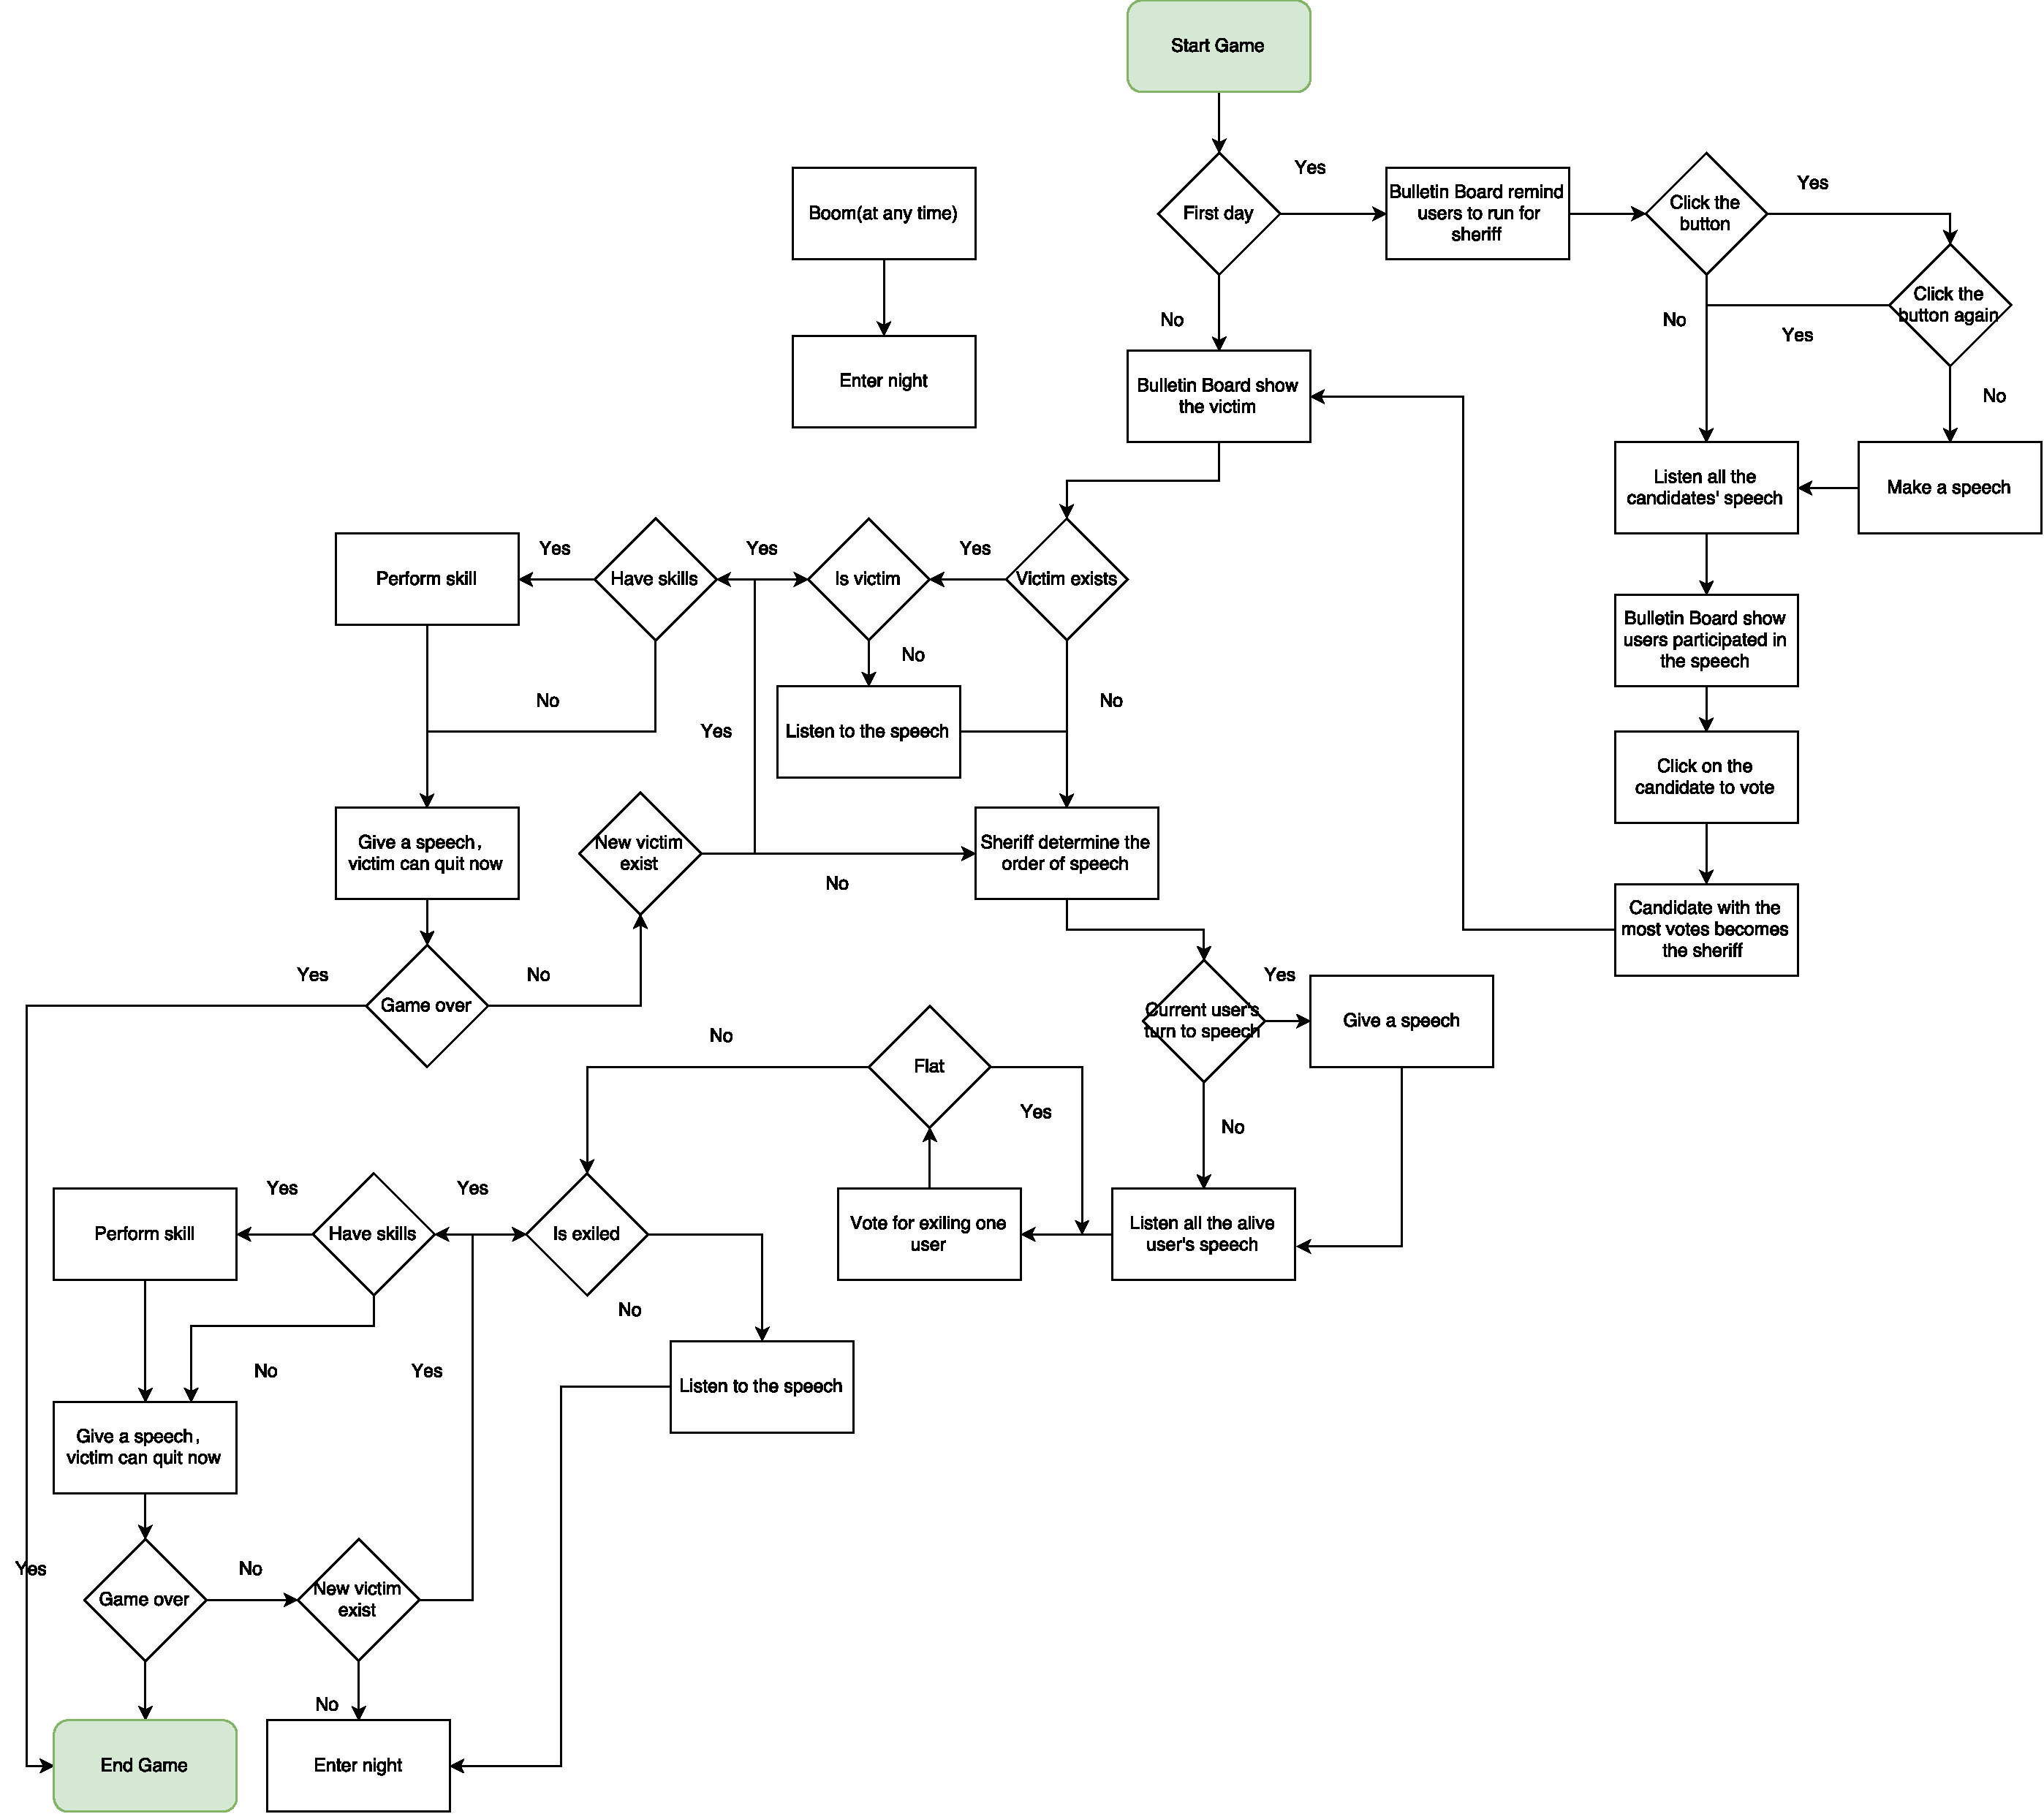
\includegraphics[width=0.9\linewidth, keepaspectratio]{func-dayphase.pdf}
\caption{Functionality: Day Phase}
\label{fig:func-dayphase}
\end{figure}

\subsubsection{Night Phase}
The main flow chart is like the Figure \ref{fig:func-nightphase}.

\begin{enumerate}
\item
Kill: Werewolf can choose one victim to kill through dragging the Paw Button in the menu to the player. All werewolf must agree on one victim. If not agreed in two rounds, there will be no victims.

\item
Poison Potion: Witch can poison a player to death through dragging the Poison Button in the menu. The skill can only be used once and can't be used with Revive Potion in the same night

\item
Revive Potion: Witch can save the victim tonight by clicking the Antidote Button in the menu. The skill can only be used once and can't be used with Poison Potion in the same night

\item
Foresee: Seer can check whether one player is a werewolf by dragging on crystal ball in the menu to the player
\end{enumerate}

\begin{figure}
\centering
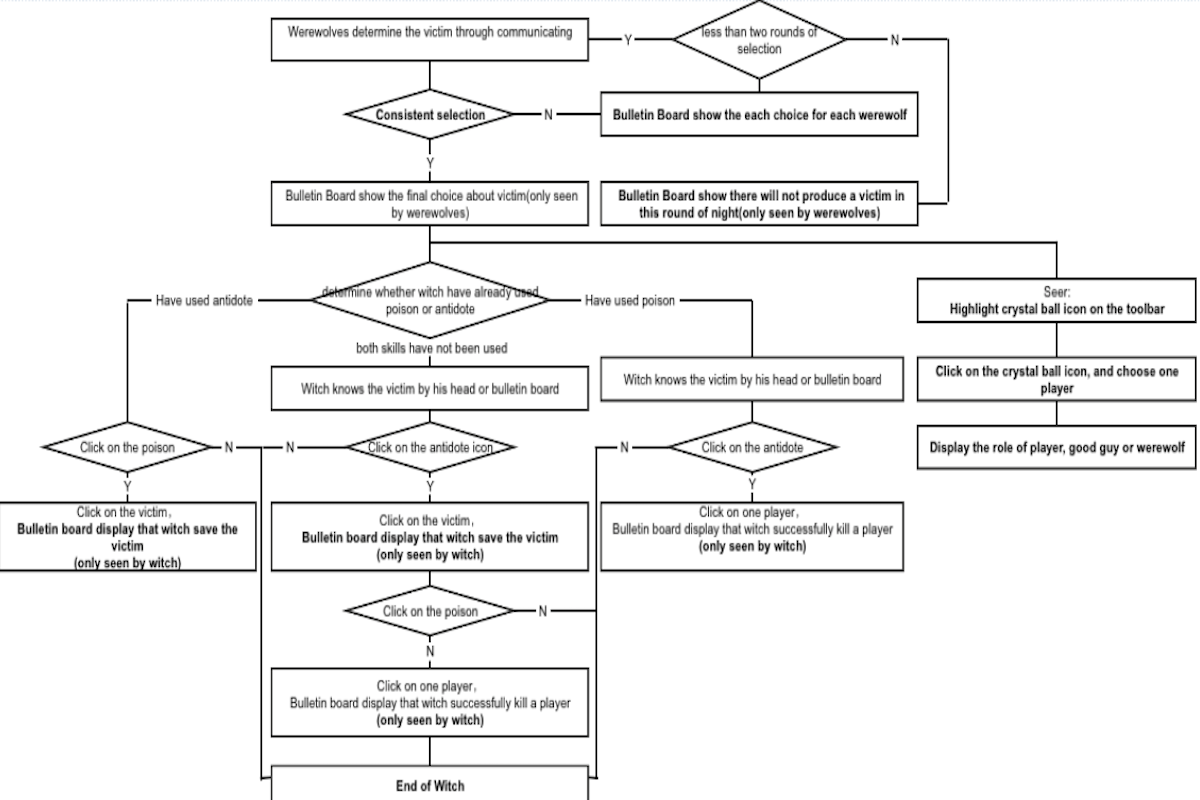
\includegraphics[width=0.9\linewidth, keepaspectratio]{func-nightphase.png}
\caption{Functionality: Night Phase}
\label{fig:func-nightphase}
\end{figure}

\section{Data Model}
\subsection{User}
User class is Django basic authenticate model. See Class Diagram in Figure \ref{fig:model-user} for detail

\begin{enumerate}
\item
first\_name: First Name
\item
last\_name: Last Name
\item
username: Username for login
\item
password: Password for login
\item
email: Email for reset password
\end{enumerate}

\begin{figure}
\centering
\begin{minipage}{.5\linewidth}
\centering
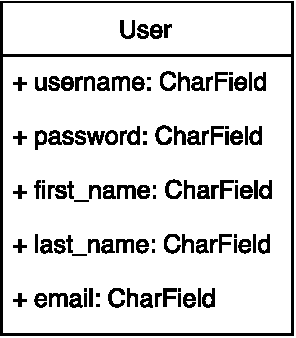
\includegraphics[width=0.7\linewidth, keepaspectratio]{model-user.pdf}
\caption{Data Model: User}
\label{fig:model-user}
\end{minipage}%
\begin{minipage}{.5\linewidth}
\centering
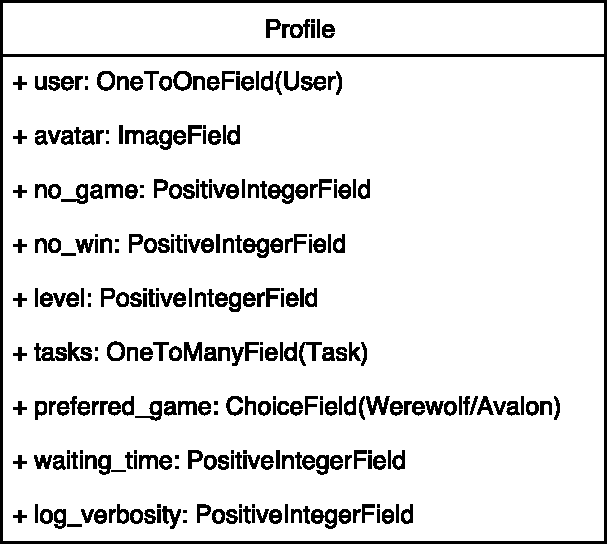
\includegraphics[width=0.9\linewidth, keepaspectratio]{model-profile.pdf}
\caption{Data Model: Profile}
\label{fig:model-profile}
\end{minipage}
\end{figure}

\subsection{Profile}
Profile class store the user data for the website. See Class Diagram in Figure \ref{fig:model-profile} for detail
\begin{enumerate}
\item
user: user relation to Django Auth User
\item
avatar: user avatar
\item
no\_game: number of games that user played
\item
no\_win: number of games that user won
\item
level: user level showing the user strength
\item
tasks: tasks assigned to user
\item
preferred\_game: user preferred game to play, shortcuts for play
\item
waiting\_time: the time user wait before his speech
\item
log\_verbosity: the log verbosity for the game state
\end{enumerate}

\subsection{Game}
Game class store the data for each game. See Class Diagram in Figure \ref{fig:model-game} for detail
\begin{enumerate}
\item
state: different states in a game, such as when state equal 0, it means the first night round
\item
role1...12: foreign key relate to Role
\end{enumerate}

\begin{figure}
\centering
\begin{minipage}{.5\linewidth}
\centering
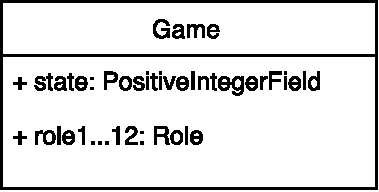
\includegraphics[width=0.7\linewidth, keepaspectratio]{model-game.pdf}
\caption{Data Model: Game}
\label{fig:model-game}
\end{minipage}%
\begin{minipage}{.5\linewidth}
\centering
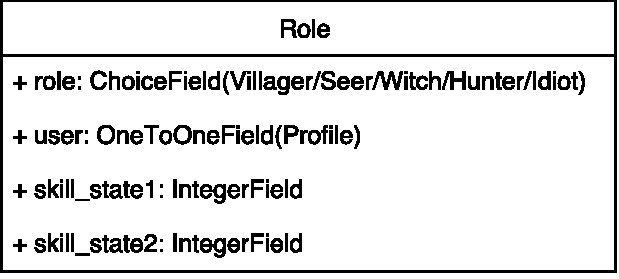
\includegraphics[width=0.9\linewidth, keepaspectratio]{model-role.pdf}
\caption{Data Model: Role}
\label{fig:model-role}
\end{minipage}
\end{figure}

\subsection{Role}
Role class store the role information. See Class Diagram in Figure \ref{fig:model-role} for detail
\begin{enumerate}
\item
role: particular role
\item
user: foreign key relate to a Profile
\item
skill\_state1: whether role have used its first skill
\item
skill\_state2: whether role have used its second skill
\end{enumerate}

\subsection{Task}
Task class store the particular task information. See Class Diagram in Figure \ref{fig:model-task} for detail
\begin{enumerate}
\item
state: if the task is in which process
\item
description: task description for user
\end{enumerate}

\begin{figure}
\centering
\begin{minipage}{.5\linewidth}
\centering
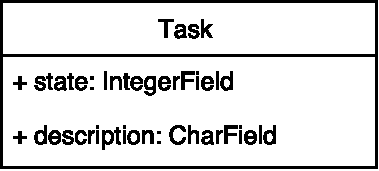
\includegraphics[width=0.7\linewidth, keepaspectratio]{model-task.pdf}
\caption{Data Model: Task}
\label{fig:model-task}
\end{minipage}%
\begin{minipage}{.5\linewidth}
\centering
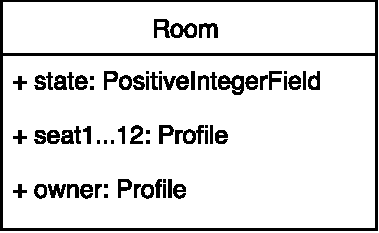
\includegraphics[width=0.7\linewidth, keepaspectratio]{model-room.pdf}
\caption{Data Model: Room}
\label{fig:model-room}
\end{minipage}
\end{figure}

\subsection{Room}
Room class store the room information. See Class Diagram in Figure \ref{fig:model-room} for detail
\begin{enumerate}
\item
state: if the room is in ready, start or end state
\item
seat1...12: foreign key to Profile, indicates which user the seat belongs to
\item
owner: foreign key to Profile, indicates which user is the room owner
\end{enumerate}

% For many users, the previous commands will be enough.
% If you want to directly input Unicode, add an Input Menu or Keyboard to the menu bar 
% using the International Panel in System Preferences.
% Unicode must be typeset using a font containing the appropriate characters.
% Remove the comment signs below for examples.

% \newfontfamily{\A}{Geeza Pro}
% \newfontfamily{\H}[Scale=0.9]{Lucida Grande}
% \newfontfamily{\J}[Scale=0.85]{Osaka}

% Here are some multilingual Unicode fonts: this is Arabic text: {\A السلام عليكم}, this is Hebrew: {\H שלום}, 
% and here's some Japanese: {\J 今日は}.



\end{document}  